\documentclass{article}

\usepackage[left=2cm,right=2cm,top=2cm,bottom=2cm]{geometry} 

\usepackage[utf8]{inputenc}   % otra alternativa para los caracteres acentuados y la "ñ"
\usepackage[           spanish % para poder usar el español
                      ,es-tabla % para los captions de las tablas
                       ]{babel}   
\decimalpoint %para usar el punto decimal en vez de coma para los números con decimales

%\usepackage{beton}
%\usepackage[T1]{fontenc}

\usepackage{parskip}
\usepackage{xcolor}

\usepackage{caption}

\usepackage{enumerate} % paquete para poder personalizar fácilmente la apariencia de las listas enumerativas

\usepackage{graphicx} % figuras
\usepackage{subfigure} % subfiguras

\usepackage{amsfonts}
\usepackage{amsmath}

\usepackage{listings}
\lstset
{ %Formatting for code in appendix
    language=python,
    basicstyle=\footnotesize,
    stepnumber=1,
    showstringspaces=false,
    tabsize=1,
    breaklines=true,
    breakatwhitespace=false,
}

\definecolor{gris}{RGB}{220,220,220}
	
\usepackage{float} % para controlar la situación de los entornos flotantes

\restylefloat{figure}
\restylefloat{table} 
\setlength{\parindent}{0mm}


\usepackage[bookmarks=true,
            bookmarksnumbered=false, % true means bookmarks in 
                                     % left window are numbered
            bookmarksopen=false,     % true means only level 1
                                     % are displayed.
            colorlinks=true,
            allcolors=blue,
            urlcolor=blue]{hyperref}
\definecolor{webblue}{rgb}{0, 0, 0.5}  % less intense blue

\usepackage[ruled,vlined]{algorithm2e}
\SetKwInOut{Parameter}{parameter}


\title{\Huge Metaheurística: Práctica Alternativa al Examen \\ Búsqueda Ramificada con Momentos \vspace{10mm}}

\author{\huge David Cabezas Berrido \vspace{10mm} \\
	\huge 20079906D \vspace{10mm} \\  
  \huge Grupo 2: Viernes \vspace{10mm} \\ 
  \huge dxabezas@correo.ugr.es \vspace{10mm}}

\begin{document}
\maketitle
\newpage
\tableofcontents
\newpage

\section{Descripción de la Metaheurística}

Diseñaremos nuestra propia metaheurística y la pondremos a prueba con el benchmark CEC'2017. Por tanto, nuestro objetivo es la optimización de parámetros
reales. Con nuestra propuesta esperamos alcanzar un buen compromiso entre exploración y explotación aprovechando la naturaleza continua del espacio
de soluciones.

\subsection{Idea general}
Nuestra metaheurística, \textbf{Búsqueda Ramificada con Momentos}, pretende ``lanzar'' soluciones que se muevan por el espacio como lo harían bombas
lanzadas desde un avión bombardeos, fragmentos que se desprenden de un cuerpo celeste o el despliegue de una sonda de una nave espacial.
Es decir, se explora el espacio ramificando o dividiendo las soluciones en otras, de
forma que las soluciones resultantes conserven la inercia de la solución de la que partieron.

\begin{figure}[H]
	\centering
	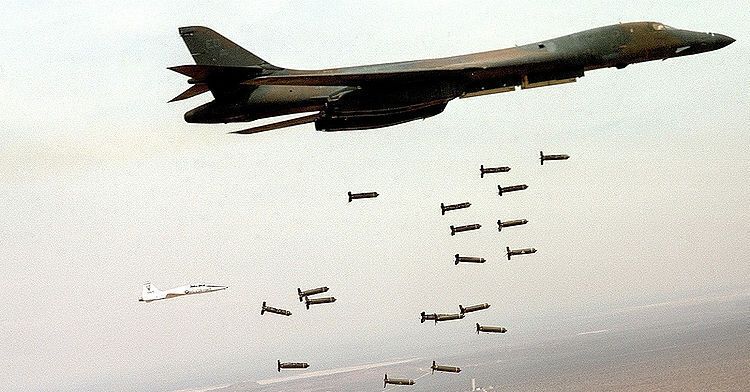
\includegraphics[width=140mm]{imgs/bombs}
	\caption{Cuando se despliegan bombas desde un avión, las bombas mantienen la inercia del movimiento del avión.}
\end{figure}

Para dar sentido a este fenómeno físico que es la conservación de la inercia ideamos una estrategia de explotación basada en momentos, similar
a la Búsqueda Local salvo que se pondera el momento de la solución con la dirección de un vecino mejor.

Las soluciones pueden ser truncadas bajo ciertas
condiciones, así que se van lanzando nuevas soluciones desde puntos aleatorios hasta agotar el número máximo de evaluaciones.

\subsection{Explicación del algoritmo}

\subsection{Detalles de implementación}
TODO: valor de los parámetros

\end{document}
